\chapter{Background}\label{ch:background}
In this chapter, we discuss some of the relevant theories for understanding our proposed framework. Section~\ref{sec:deep_learning_basics} discusses some of the key concepts of different deep learning algorithms, such as convolutional neural networks, and recurrent neural networks. We also illustrate different types of regularization and normalization techniques required to train our proposed network. In Section~\ref{sec:pose_estimation} we will present an overview of the human pose estimation algorithms employing deep learning. 


%-------------------------------------------------------------------------
\section{Deep Learning Basics} \label{sec:deep_learning_basics}
\subsection{Deep learning}
Machine Learning (\gls{ml}) is a field of \gls{ai} that utilizes statistical techniques to learn hidden patterns from available data and make decisions on unseen records. The core task of a \gls{ml} algorithm is to first build a general model based on the probability distribution of training examples, and then generalizes its experience on unseen examples. The process of learning is highly dependent on the quality of data representation.

Deep Learning (\gls{dl}) is an advanced branch of the \gls{ml} field that aims to discover the complex representation out of simpler representations. \gls{dl} methods are typically based on artificial neural networks that consist of multiple hidden layers with nonlinear processing units. The word \textit{deep} refers to the multiple hidden layers that are used for transforming the data representation. Using the concept of feature learning, each hidden layer of neural network maps its input data into a new representation. The succeeding layer tends to capture a higher level of abstraction from the less abstract concept in the preceding layer and the hierarchy of learned features in multiple levels are finally mapped to the output of the \gls{ml} task (e.g., classification and regression) in an unified framework.


\gls{dl} architectures are divided into two broad categories: (1) unsupervised learning approaches including restricted boltzmann machines (RBMs), deep autoencoders, and generative adversarial networks (GANs), (2) supervised learning approaches including deep neural networks (\gls{dnn}s), convolutional neural networks (\gls{cnn}s), and recurrent neural networks (\gls{rnn}s).


Although, (\gls{dnn}s) automatically extract rich and high level features which is needed for feature engineering, one of the most time-consuming parts of machine learning practice, increasing the depth does not necessarily improve their performance. Firstly, because they easily suffer from the overfitting problem, which means the model does not generalize well to test cases. Secondly, because they are more difficult to train and more training data is needed for convergence. To alleviate this problem special types of deep neural networks, e.g., \gls{cnn}s and \gls{rnn}s are introduced.


Some of the real-world applications of Deep Learning include image recognition~\cite{Krizhevsky_12}, image captioning~\cite{Mao_15}, machine translation~\cite{kal_13}, video classification~\cite{karpathy_14} and speech recognition~\cite{graves_13}. This thesis aims to contribute to this growing area of research by exploring the potential power of deep learning techniques in gait recognition. 


\begin{figure}
	\centering
	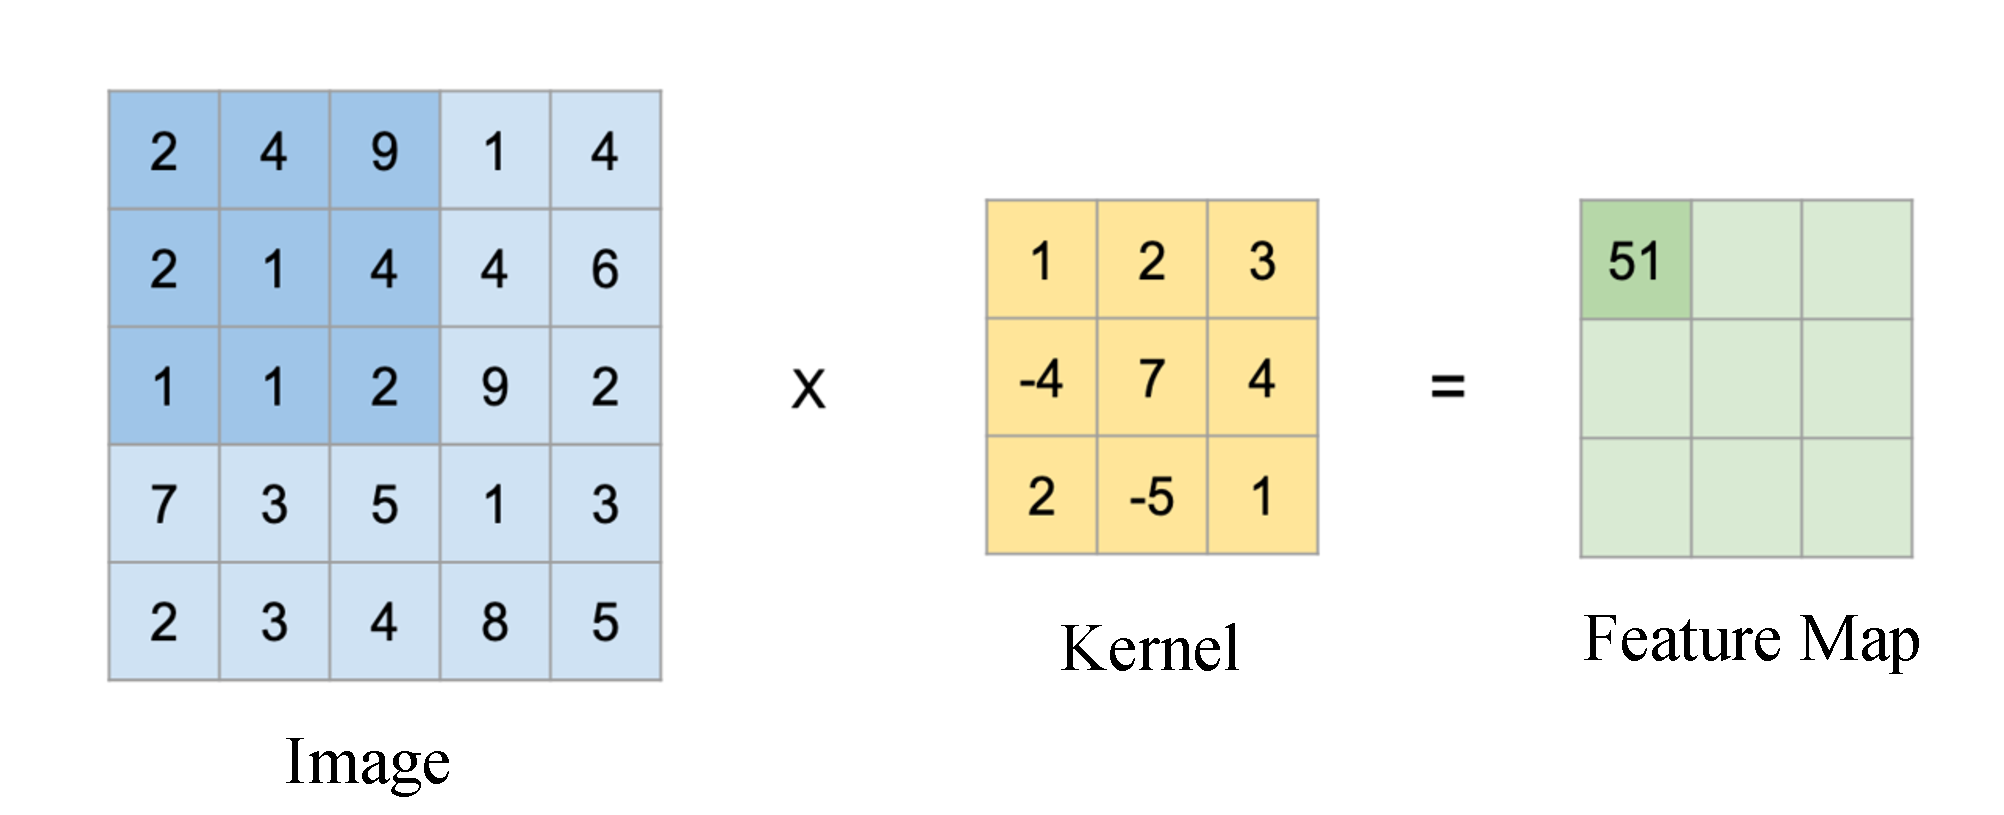
\includegraphics[width=0.8\textwidth]{figures/convolution.eps}
	\caption[Computing output activation of a convolutional layer]
	{Computing output activation of a convolutional layer \label{fig:convolution}}
\end{figure}


\subsection{Convolutional Neural Networks}
Convolutional neural networks (ConvNets or CNNs) are a category of neural networks which are proven to be very effective in areas such as image recognition~\cite{Krizhevsky_12}, video classification~\cite{karpathy_14}, and action recognition~\cite{Tran_15}. They were inspired by biological processes~\cite{Hubel_68} in that the connectivity pattern between neurons resembles the organization of the animal visual cortex. Individual neurons respond to stimuli only in a restricted region of the visual field known as the \textit{receptive field}. The receptive fields of different neurons partially overlap such that they cover the entire visual field. 

When the input, e.g. images, have a local topological structure that does not depend on the specific location in the global reference system, a dense connectivity pattern might be wasteful. It is usually preferable to be able to exploit the data structure. Firstly, because adapting the connectivity pattern according to the structure of the data reduces total number of parameters and hence number of the  operations performed by the network, which consequently reduces the risk of overfitting. Additionally, it also reduce the memory usage and the computation time. Secondly, constraining the connectivity pattern can have the effect of forcing the network to focus on what is important, yielding faster training and better performance.

\gls{cnn}s exploit this understanding of the data by applying the same pattern detector at every locations in the image. This is formally done through a \textit{convolution}, a signal processing operation that superimposes a pattern detector usually called a \textit{filter} or \textit{kernel} on different locations of the image and emits an activation in each position to produce a matrix of activations, typically referred to as \textit{feature map}. 

Let, $\mathbf{X}$ is a two-dimensional image and $\mathbf{W}$ is the weight matrix, also called a ’kernel’, then the convolution operation can be defined as 

\begin{equation}
(W \ast X)(i, j) = \sum_{m}\sum_{n} X(m, n) W (i - m, j - n)
\end{equation}

Intuitively, the output of the convolutional layer is formed by sliding the weight matrix over the image and computing the dot product (see Figure~\ref{fig:convolution}). In any real-world application, it would be common to apply multiple kernels at once with the same convolution hence obtaining a tensor of feature maps.

\begin{figure}
	\centering
	\includegraphics[width=0.9\textwidth]{figures/RNN_unrolled.pdf}
	\caption[A typical rolled representation of a recurrent neural network]
	{(a) A typical rolled representation of a recurrent neural network. (b) Unrolled recurrent neural network for $t$\% timesteps. [Image courtesy Chris Olah~\cite{colah_15}]\label{fig:RNN_unrolled}}
\end{figure}



\subsection{Recurrent Neural Networks} 
Recurrent neural networks (\gls{rnn}s) are a type of artificial neural networks (\gls{ann}s) where the output from the previous step is fed as input to the current step. It achieves state-of-the-art performance on various tasks in different domains such as language modeling~\cite{mikolov_12}, speech recognition~\cite{graves_13}, and machine translation~\cite{kal_13}.  

RNNs implement feedback loops (see Figure~\ref{fig:RNN_unrolled}a) that propagate some information from one timestep to the next. It might be confusing in practice to put a loop in an \gls{ann} and backpropagate through it. To better comprehend how RNNs work it is useful to consider its behavior explicitly by \emph{unrolling} the RNN, as shown in Figure~\ref{fig:RNN_unrolled}b.



\begin{figure}
	\centering
	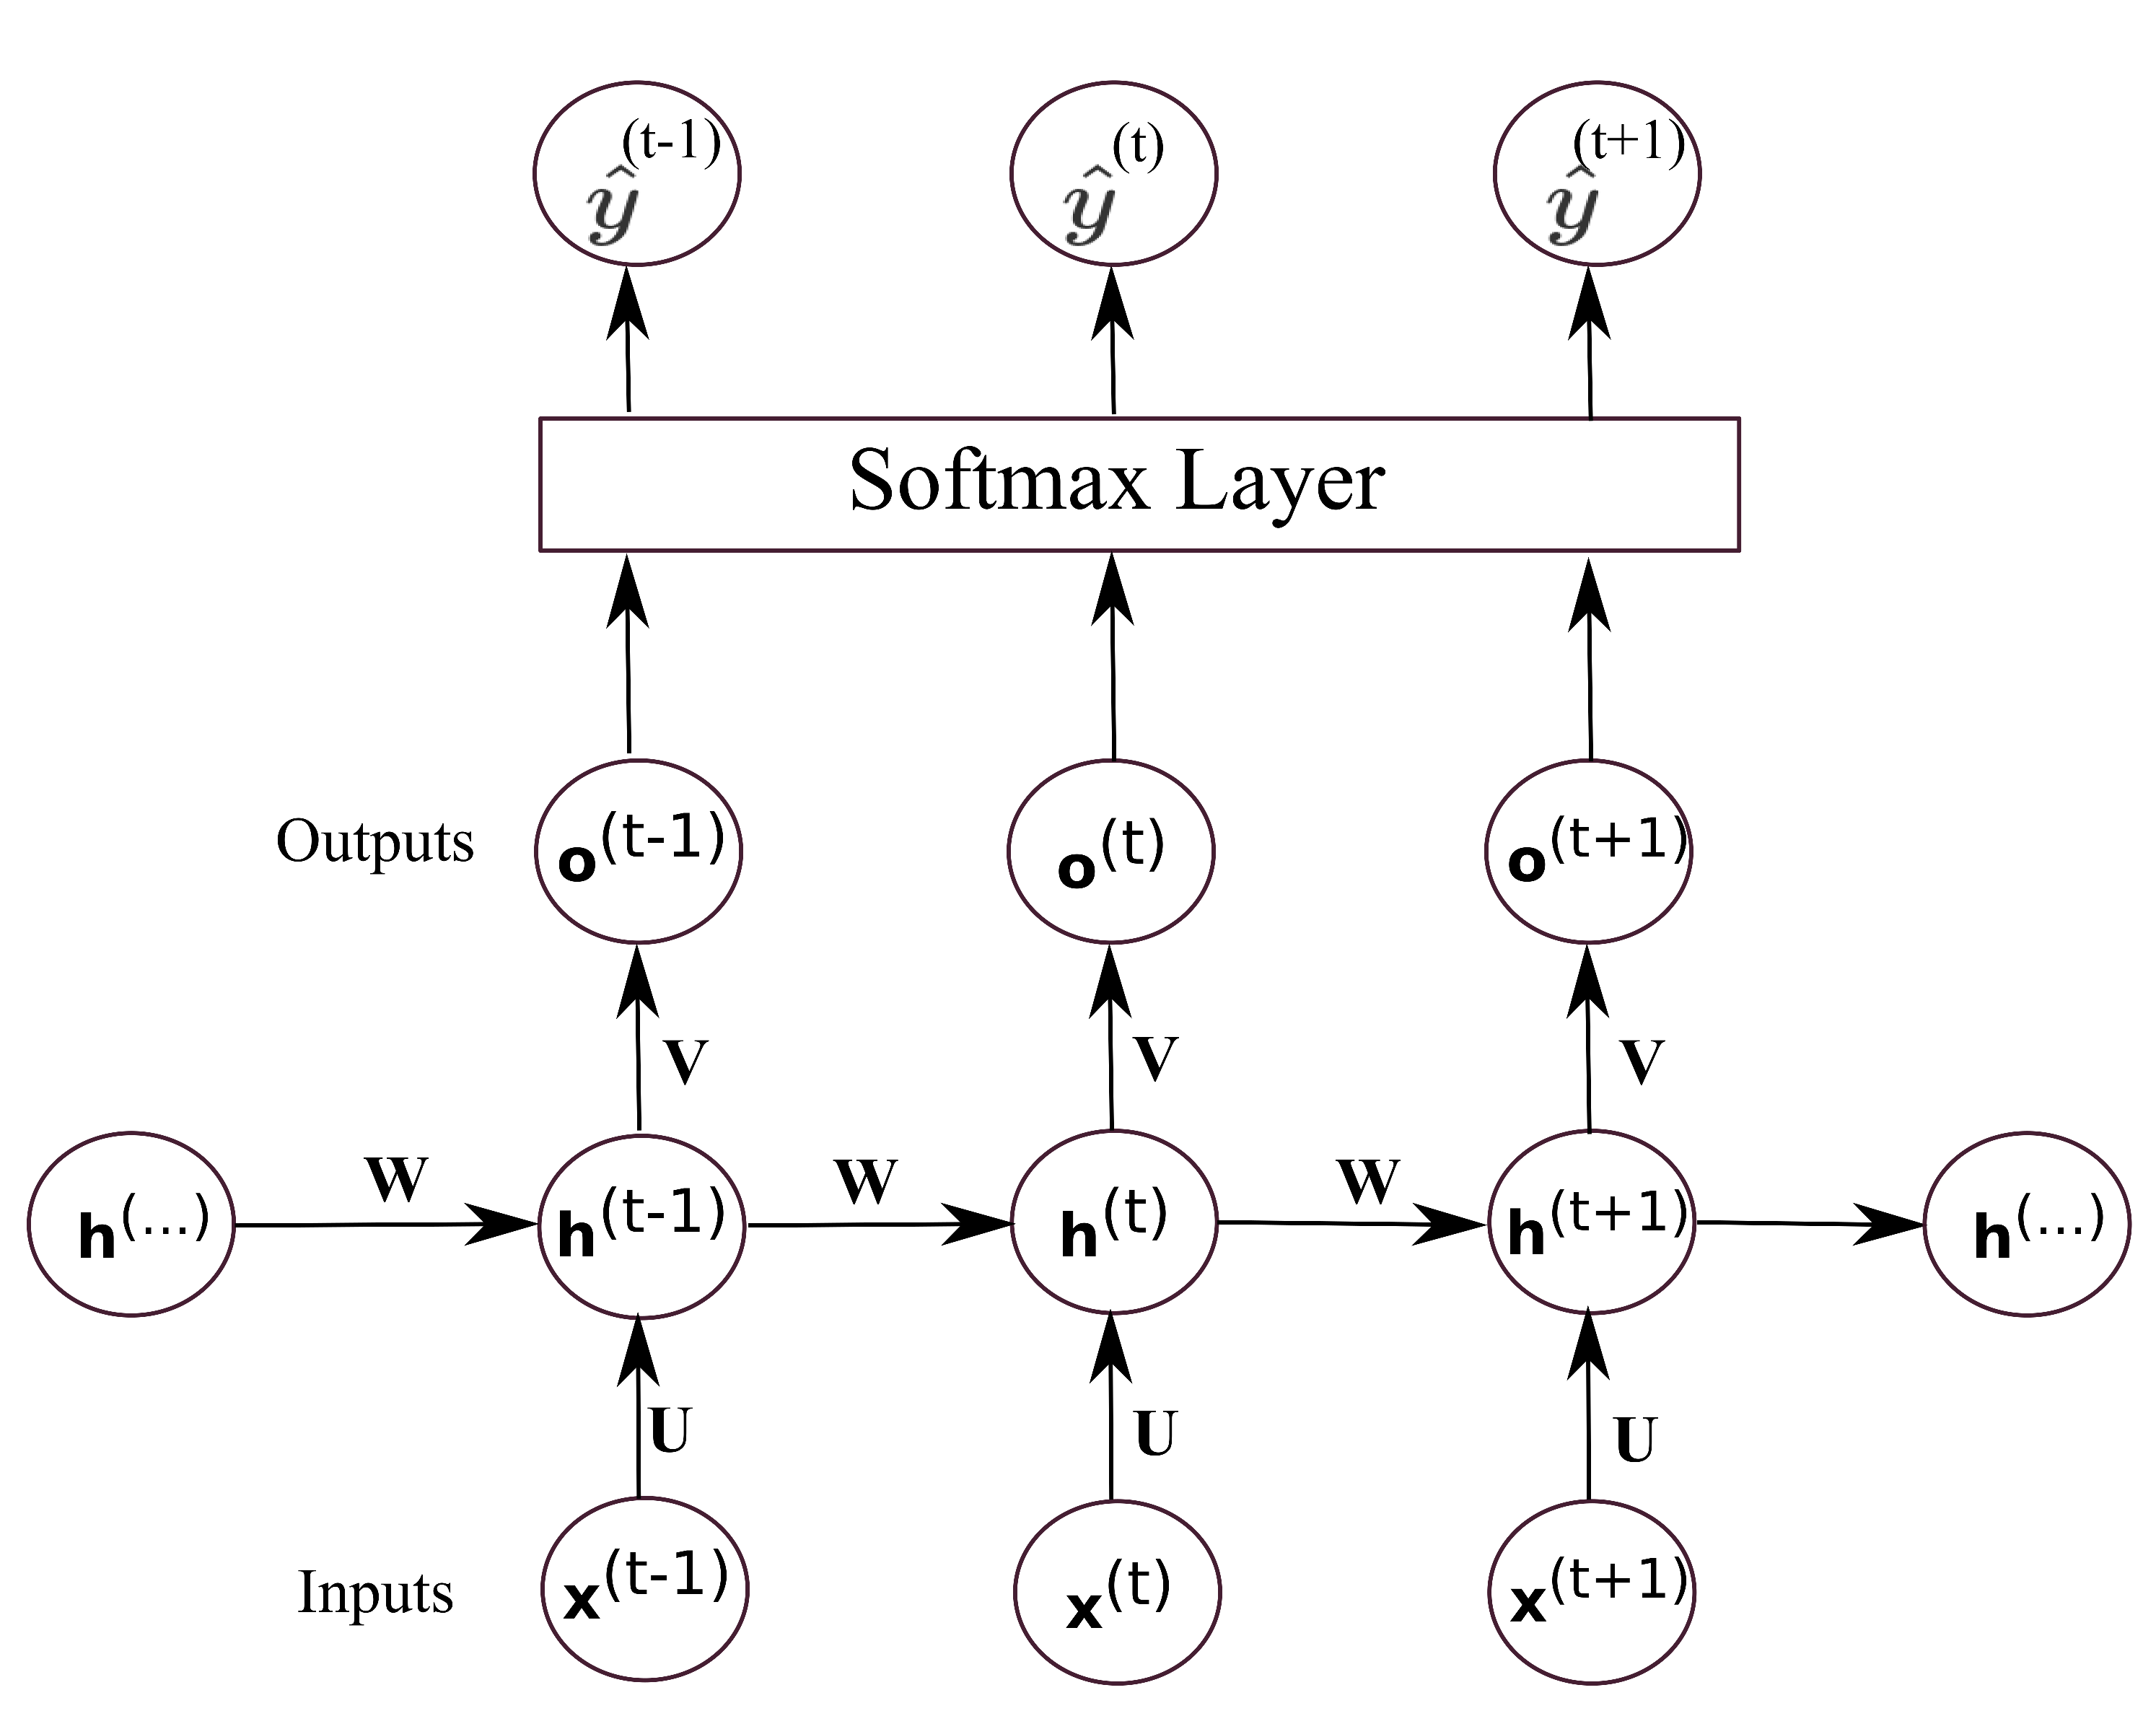
\includegraphics[width=0.7\textwidth]{figures/rnn_unrolling.eps}
	\caption{The computational graph of a unrolled recurrent neural network that maps an input sequence of $ \textbf{x}$ values to a corresponding sequence of output $\textbf{o}$ values \label{fig:RNN_unrolling}}
\end{figure}

The forward propagation equations of \gls{rnn} are depicted in Figure~\ref{fig:RNN_unrolling}. Forward propagation begins with a specification of the initial state $ \textbf{h}^{(0)} $. Then, for each timestep from $ t $ we apply the following update equations:

\begin{equation} \label{rnn_unroll}
\begin{split}
	\textbf{a}^{(t)} &= \textbf{b} + \textbf{W} \cdot \textbf{h}^{(t-1)} + \textbf{U} \cdot \textbf{x}^{(t)} \\
	\textbf{h}^{(t)}&=\tanh(\textbf{a}^{(t)})\\
	\textbf{o}^{(t)}&= \textbf{c} + \textbf{V} \cdot \textbf{h}^{(t)} \\
	{\hat{\textbf{y}}}^{(t)} &= softmax(\textbf{o}^{(t)})
\end{split}
\end{equation}

Here, the parameters are the bias vectors $ \textbf{b} $ and $ \textbf{c} $ along with the weight matrices $\textbf{U}$, $\textbf{V}$ and $\textbf{W}$, respectively, for input-to-hidden, hidden-to-output and hidden-to-hidden connections. The activation of an RNN (see Figure ~\ref{fig:RNN_unrolling}) at time $t$ depends on the input at time $t$ as well as on the information coming from the previous step $t-1$. \gls{rnn}s have a very simple internal structure, that usually amounts to applying some affine transformation to the input and to the previous output, and computing some non-linearity (typically a $tanh$) of their sum.

The sequential information is preserved in the recurrent network's hidden state, which manages to span many timesteps as it cascades forward to affect the processing of each new example. It is finding correlations between events separated by many moments, and these correlations are called \textit{long-term dependencies}, because an event downstream in time depends upon, and is a function of, one or more events that came before. One way to think about RNNs is that they applies the same model to each timestep of the sequence or, equivalently, applies different models at each timestep which share their weights. 

For training these networks, it is required to unroll the computation graph and use the backpropagation algorithm to proceed from the most recent timestep. This algorithm is usually referred to as \emph{Backpropagation through time} (\gls{bptt}). The problem of \gls{bptt} is that it requires the application of the chain rule all the way from the current timestep to $t = 0$ to propagate the gradients.  This results in a long chain of products that can easily go to infinity or become zero if the elements of the multiplication are greater or smaller than $1$ respectively ~\cite{Bengio_94}. These two issues, i.e., going to infinity and becoming zero, are known in the literature as \emph{exploding gradient} and \emph{vanishing gradient}~\cite{Hochreiter_01} problem respectively. The first one can be partially addressed by \emph{clipping the gradient} when it becomes too large, but the second is not easy to overcome and can make training these kind of models very hard.


\subsection{Long Short-Term Memory}
\begin{figure}[t]
	\centering
	\includegraphics[width=0.7\textwidth]{figures/LSTM.pdf}
	\caption[A long short-term memory (LSTM)]
	{A long short-term memory (LSTM). [Image courtesy Chris Olah~\cite{colah_15}]\label{fig:LSTM}}
\end{figure}

Long short-term memory (\gls{lstm}) networks (Figure~\ref{fig:LSTM}) have been proposed to solve the problems of RNNs in modeling long-term dependencies. LSTMs have been designed to have an internal memory, or~\emph{state}, that can be updated at each timestep. As opposed to vanilla \gls{rnn}, this internal memory allows LSTM to separate their output from the information they want to carry over into the future steps.

\begin{figure}[t]
	\centering
	\includegraphics[width=0.6\textwidth]{figures/LSTM_state.pdf}
	\caption[The internal state of LSTMs]
	{The internal state of LSTMs. [Image courtesy Chris Olah~\cite{colah_15}]\label{fig:LSTM_state}}
\end{figure}

Figure \ref{fig:LSTM_state} highlights the internal memory path. From the figure it can be observed that how the internal memory of the previous timestep $\mathbf{c}_{t-1}$ is carried over to the current timestep where it is updated through a multiplicative and an additive interaction and concurs to determine the current state of the memory $\textbf{c}_t$. Thereafter, this state once again, propagated to the next timestep.


\begin{figure}[p]
	\centering
	\includegraphics[width=0.6\textwidth]{figures/LSTM_forget_gate.pdf}
	\caption[The LSTM forget gate]
	{The LSTM forget gate. [Image courtesy Chris Olah~\cite{colah_15}]\label{fig:LSTM_forget_gate}}
\end{figure}
\begin{figure}[p]
	\centering
	\includegraphics[width=0.6\textwidth]{figures/LSTM_input_gate.pdf}
	\caption[The LSTM input gate]
	{The LSTM input gate. [Image courtesy Chris Olah~\cite{colah_15}]\label{fig:LSTM_input_gate}}
\end{figure}
\begin{figure}[p]
	\centering
	\includegraphics[width=0.6\textwidth]{figures/LSTM_output_gate.pdf}
	\caption[The LSTM output gate]
	{The LSTM output gate.[Image courtesy Chris Olah~\cite{colah_15}]\label{fig:LSTM_output_gate}}
\end{figure}


\gls{lstm}s interact with memory through \emph{gate}, a computational node, that determines the behavior of the model. The \emph{forget~gate}, as shown in Figure~\ref{fig:LSTM_forget_gate}, determines how much of the previous step's memory to forget or, equivalently, how much of the previous state to retain.  This is modeled through a sigmoid layer ($\sigma$) that takes the current input $\textbf{x}_t$ and the output of the previous step $\mathbf{h}_{t-1}$ and produces an activation vector between $0$ and $1$.  This activation is multiplied by the previous state $\mathbf{c}_{t-1}$ and results in an intermediate memory state where some of the activations can be weaker than those in $\mathbf{c}_{t-1}$ and some others are potentially zeroed out.

The forget gate allows the LSTM to discard information that is not relevant anymore. 
\begin{equation}\label{eq:LSTM_forget_gate}
\mathbf{f}_t = \sigma\left(\mathbf{W}_f \cdot \mathbf{x}_t + \mathbf{U}_f \cdot \mathbf{h}_{t-1} + \mathbf{b}_f \right),
\end{equation}

Again, \gls{lstm}s have a mechanism to add new information to the memory. This behavior is controlled by an \emph{input gate} (Figure \ref{fig:LSTM_input_gate}) that modulates the amount of the current input that is going to be stored in the memory. This operation is split over two computation paths: similarly to the forget gate, the input gate takes the current input $\mathbf{x}_t$ and the output of the previous step $\mathbf{h}_{t-1}$ and exploits a sigmoid layer to produce an activation vector between $0$ and $1$. Simultaneously, a $tanh$ layer generates a state update $\mathbf{\tilde c}_t$ between $-1$ and $1$. This is governed by the following equations:

\begin{equation}\label{eq:LSTM_input_gate}
\begin{split}
\mathbf{i}_t &= \sigma\left(\mathbf{W}_i \cdot \mathbf{x}_t + \mathbf{U}_i \cdot \mathbf{h}_{t-1} + \mathbf{b}_i \right)\\
\mathbf{\tilde c}_t &= tanh \left(\mathbf{W}_c \cdot \mathbf{x}_t + \mathbf{U}_c \cdot \mathbf{h}_{t-1} + \mathbf{b}_c \right)
\end{split}
\end{equation}

The input gate modulates how much of this state update will be applied to the old state to generate the current state. The forget gate $\mathbf{f}_t$ and the input gate $\mathbf{i}_t$, together with the state update $\mathbf{\tilde c}_t$ and the previous state $\mathbf{c}_{t-1}$ fully determine the state at time $t$. 

\begin{equation}\label{eq:LSTM_state_update}
\mathbf{c}_t = \mathbf{f}_t \circ \mathbf{c}_{t-1} + \mathbf{i}_t \circ \mathbf{\tilde c}_t
\end{equation}

Here, the symbol $\circ$ denotes \textit{Hadamard product}, i.e., the element-wise multiplication between two identical shaped matrices. The last gate of \gls{lstm} is the \emph{output~gate} (Figure~\ref{fig:LSTM_output_gate}) $\mathbf{o}_t$ that, as the name reveals, manipulates the output of the LSTM at time $t$. The usual sigmoid layer determines the state of the output gate and the memory resulting from the transformations due to the forget and input gates goes through a $tanh$ nonlinearity and is multiplied by the output gate to finally produce the output.

\begin{equation}\label{eq:LSTM_output_gate}
\begin{split}
\mathbf{o}_t &= \sigma\left(\mathbf{W}_o \cdot \mathbf{x}_t + \mathbf{U}_o \cdot \mathbf{h}_{t-1} + \mathbf{b}_o \right)\\
\mathbf{h}_t &= \mathbf{o}_t \circ tanh \left(\mathbf{c}_t\right)
\end{split}
\end{equation}


\begin{figure}
	\centering
	\includegraphics[width=0.6\textwidth]{figures/GRU.pdf}
	\caption[Gated Recurrent Units (GRUs)]
	{Gated recurrent units (GRUs). [Image courtesy Chris Olah~\cite{colah_15}]\label{fig:GRU}}
\end{figure}

\subsection{Gated Recurrent Unit}\label{sec:GRU}
Cho \textit{et al.}~\cite{Cho_14} proposed a new kind of RNN called gated recurrent unit (\gls{gru}), as shown in Figure~\ref{fig:GRU}, with less gates than \gls{lstm} and a different internal structure. In \gls{gru}s the forget and input gates are coupled into an~\emph{update gate} $\mathbf{z}_t$.  The memory and output are also merged into a single state and the internal structure is modified to cope with these changes. Figure~\ref{fig:GRU} shows the internal structure of a GRU unit.

The \textit{update gate} $\mathbf{z}_t$ for timestep $t$ helps the model to determine how much of the information from the previous timestep needs to be passed along the future.  It is analogous to the output gate in an LSTM cell.
\begin{equation}
\mathbf{z}_t = \sigma \left(\mathbf{W}_z \cdot \mathbf{x}_t + \mathbf{U}_z \cdot \mathbf{h}_{t-1} + \mathbf{b}_z\right)
\end{equation}

On the other hand, \textit{reset gate} in GRU is used to decide how much of the past information needs to forget. It is analogous to the combination of the input gate and the forget gate in an LSTM cell.
\begin{equation}
\mathbf{r}_t = \sigma \left(\mathbf{W}_r \cdot \mathbf{x}_t + \mathbf{U}_r \cdot \mathbf{h}_{t-1} + \mathbf{b}_r\right)
\end{equation}

GRU has also a new memory content which will use the reset gate to store the relevant information from the past
\begin{equation}
\mathbf{\tilde h}_t = tanh \left(\mathbf{W}_h \cdot \mathbf{x}_t + \mathbf{U}_h \cdot (\mathbf{r}_t \circ \mathbf{h}_{t-1}) + \mathbf{b}_h\right)
\end{equation}

In the last step, the GRU calculates the current information $\mathbf{h}_t$ from the update gate ($\mathbf{z}_t$), previous information ($\mathbf{h}_{t-1}$), and memory content ($\mathbf{\tilde h}_t$) and passes it down to the network. 
\begin{equation}
\mathbf{h}_t = \mathbf{z}_t \circ \mathbf{h}_{t-1} + (1 - \mathbf{z}_t) \circ \mathbf{\tilde h}_t.
\end{equation}

Therefore, the differences between LSTM unit and GRU are:
\begin{itemize}
	\item GRUs have 2 gates while LSTMs have 3 gates
	\item GRUs do not have any internal memory in contrast to LSTMs
	\item Nonlinearity is not applied when computing the output of GRUs
\end{itemize}

The advantage of \gls{gru}s over \gls{lstm}s is the smaller number of gates that make them less memory as well as computationally intense, which is often a critical aspect for \gls{ann}s. Therefore, GRU involves less computation compared with LSTM while keeping similar performance and improving the efficiency of the original \gls{rnn}s. That's why, \gls{gru} has shown better classification performance on smaller datasets~\cite{Chung_14}.

\begin{figure}[t]
	\centering
	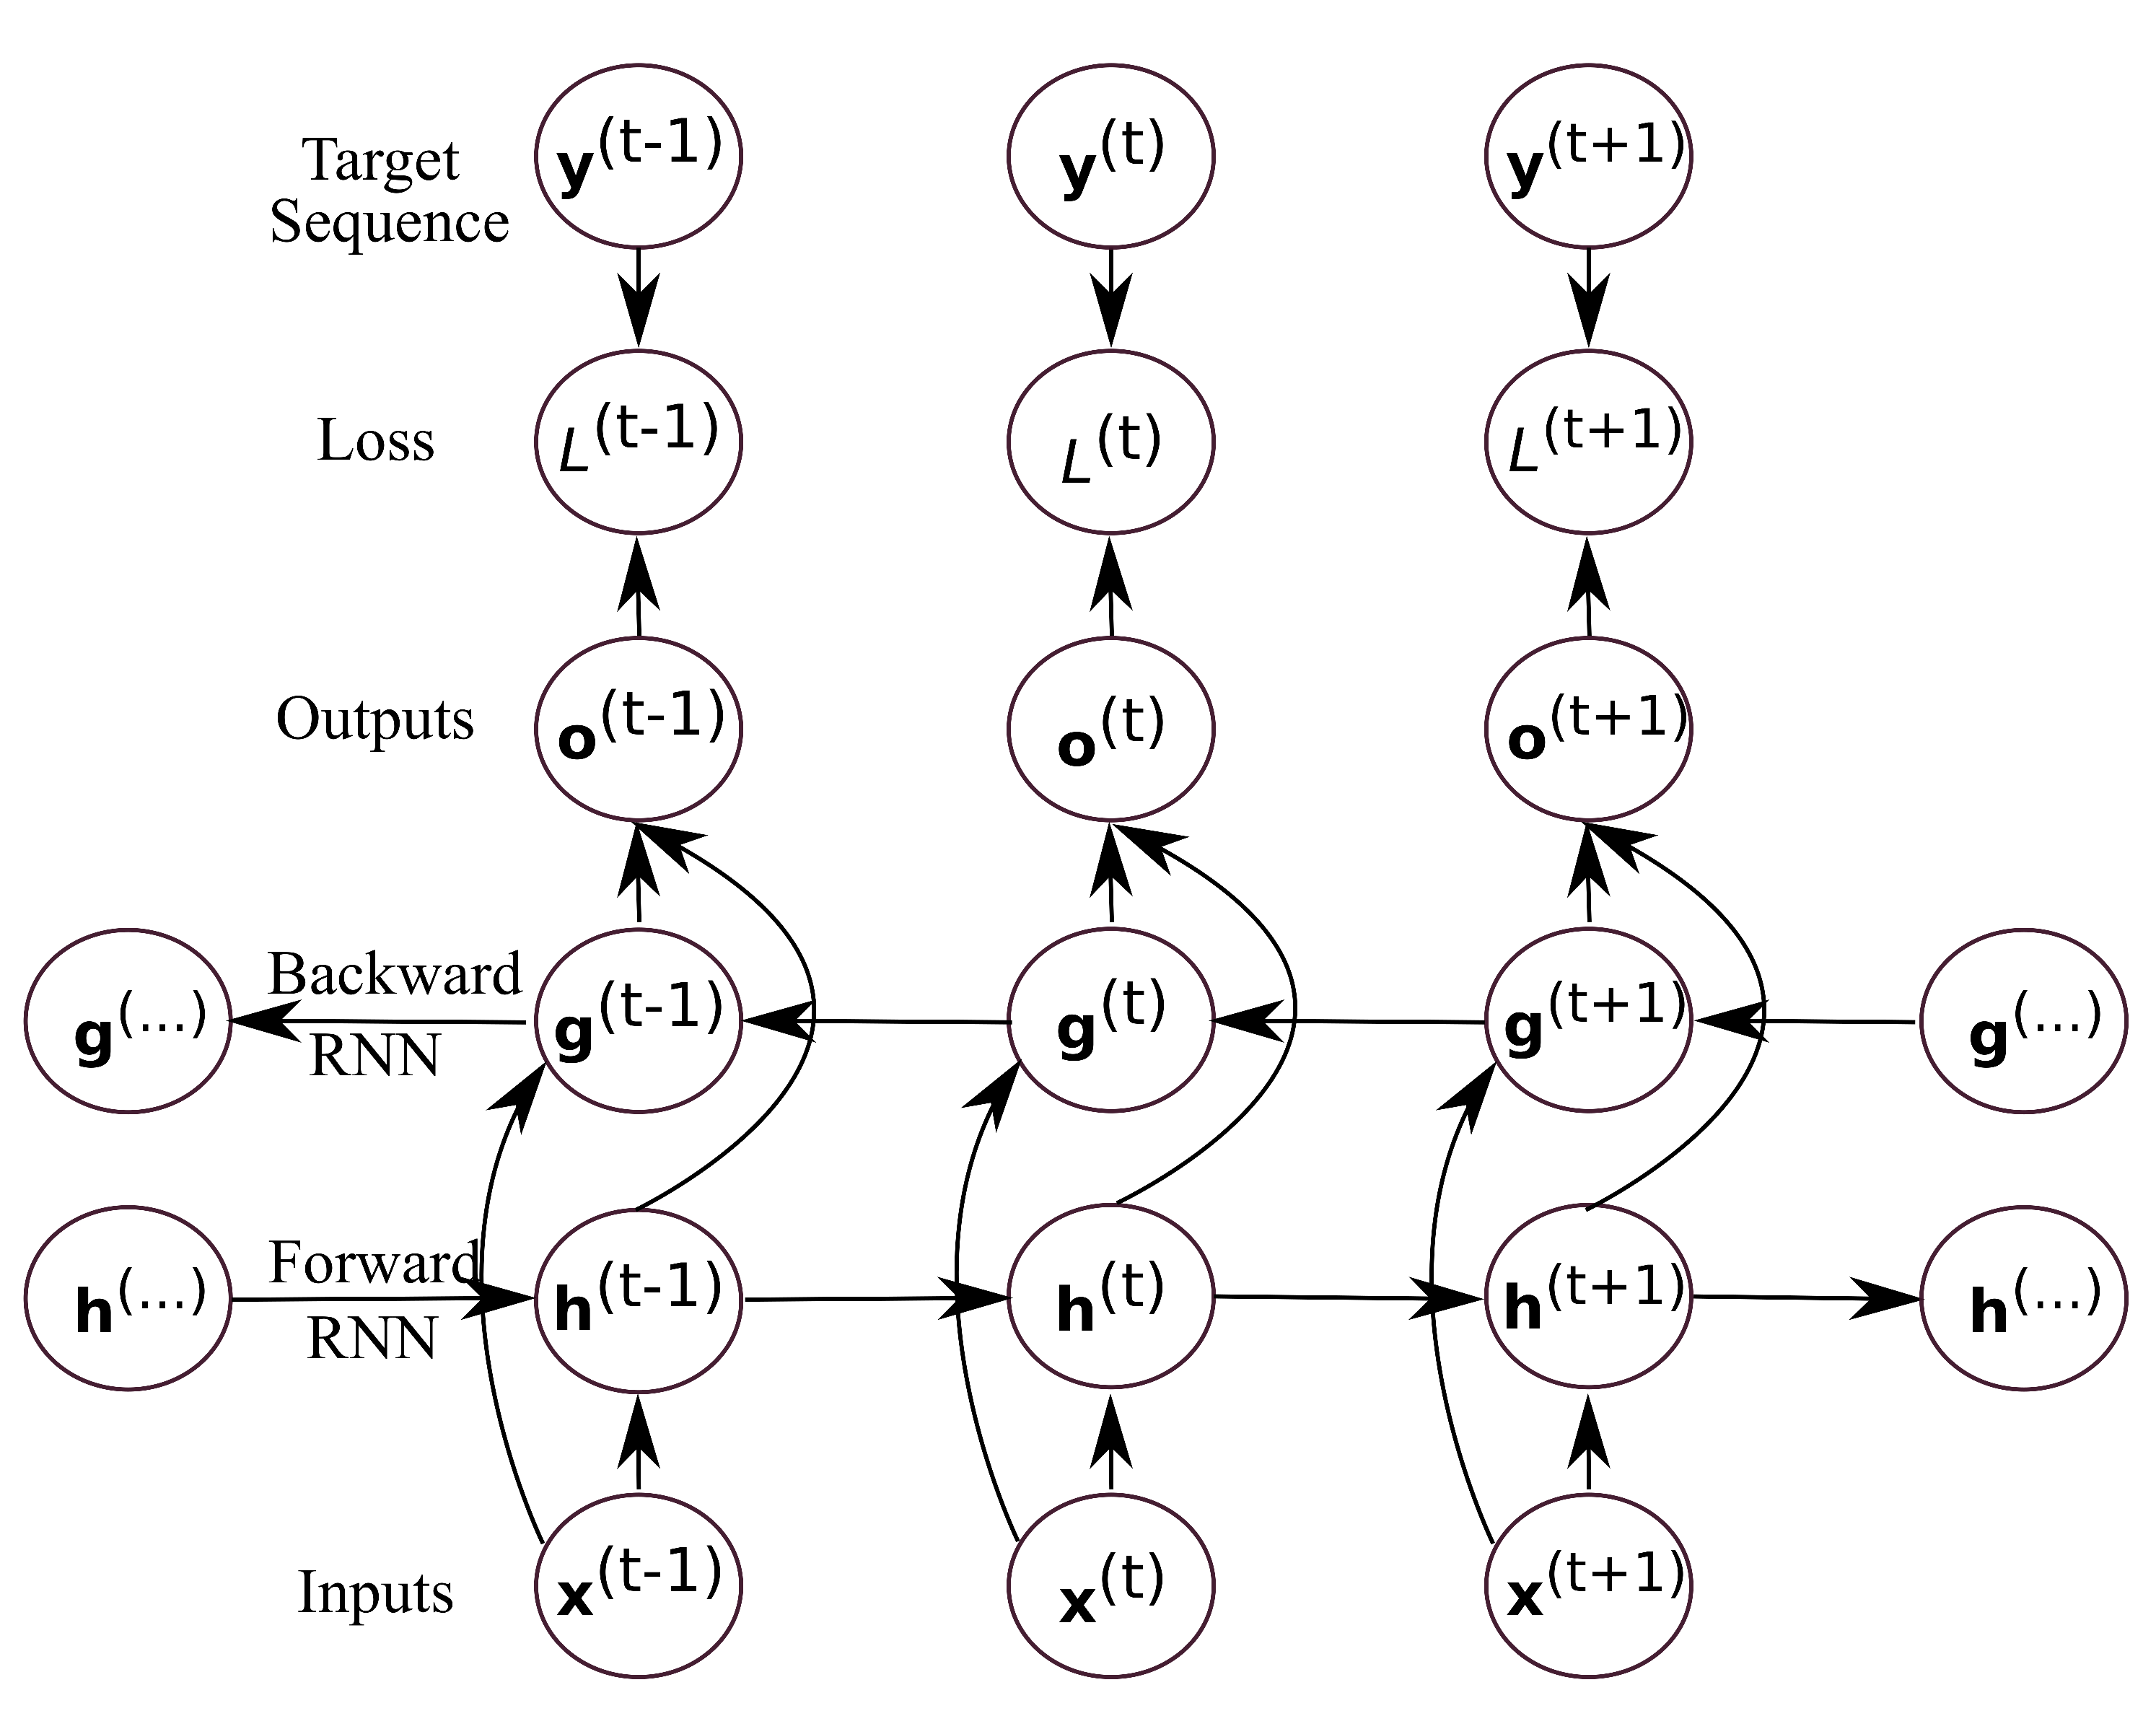
\includegraphics[width=0.8\textwidth]{figures/brnn.eps}
	\caption{The architecture of a vanilla bidirectional recurrent neural network \label{fig:bidirectional_rnn}}
\end{figure}



\subsection{Bidirectional RNNs}
Bidirectional recurrent neural networks (\gls{brnn}s)~\cite{Schuster_97} connect two hidden layers running in opposite directions into a single output, allowing them to receive information from both past and future states. Here, the input sequence is fed in normal time order for one network, and in reverse time order for another. The outputs of the two networks are usually concatenated at each timestep. So, this type of structure allows the networks to have both backward and forward information about the sequence at every timestep. \gls{brnn}s are especially useful when the context of the input is needed. For example, in handwriting recognition~\cite{Graves_08}, the performance can be enhanced by knowledge of the letters located before and after the current letter.  A vanilla architecture of the \gls{brnn} is illustrated in Figure~\ref{fig:bidirectional_rnn}. 


\subsubsection{Bidirectional GRU}
In a  bidirectional GRU (\gls{bigru}) consists of 2 vanilla unidirectional \gls{gru}s stacked side by side, but the second GRU reads the input sequence from the opposite direction. Figure~\ref{fig:bidirectional_gru} illustrates the basic architecture of a Bidirectional GRU. 
\begin{figure}[t]
	\centering
	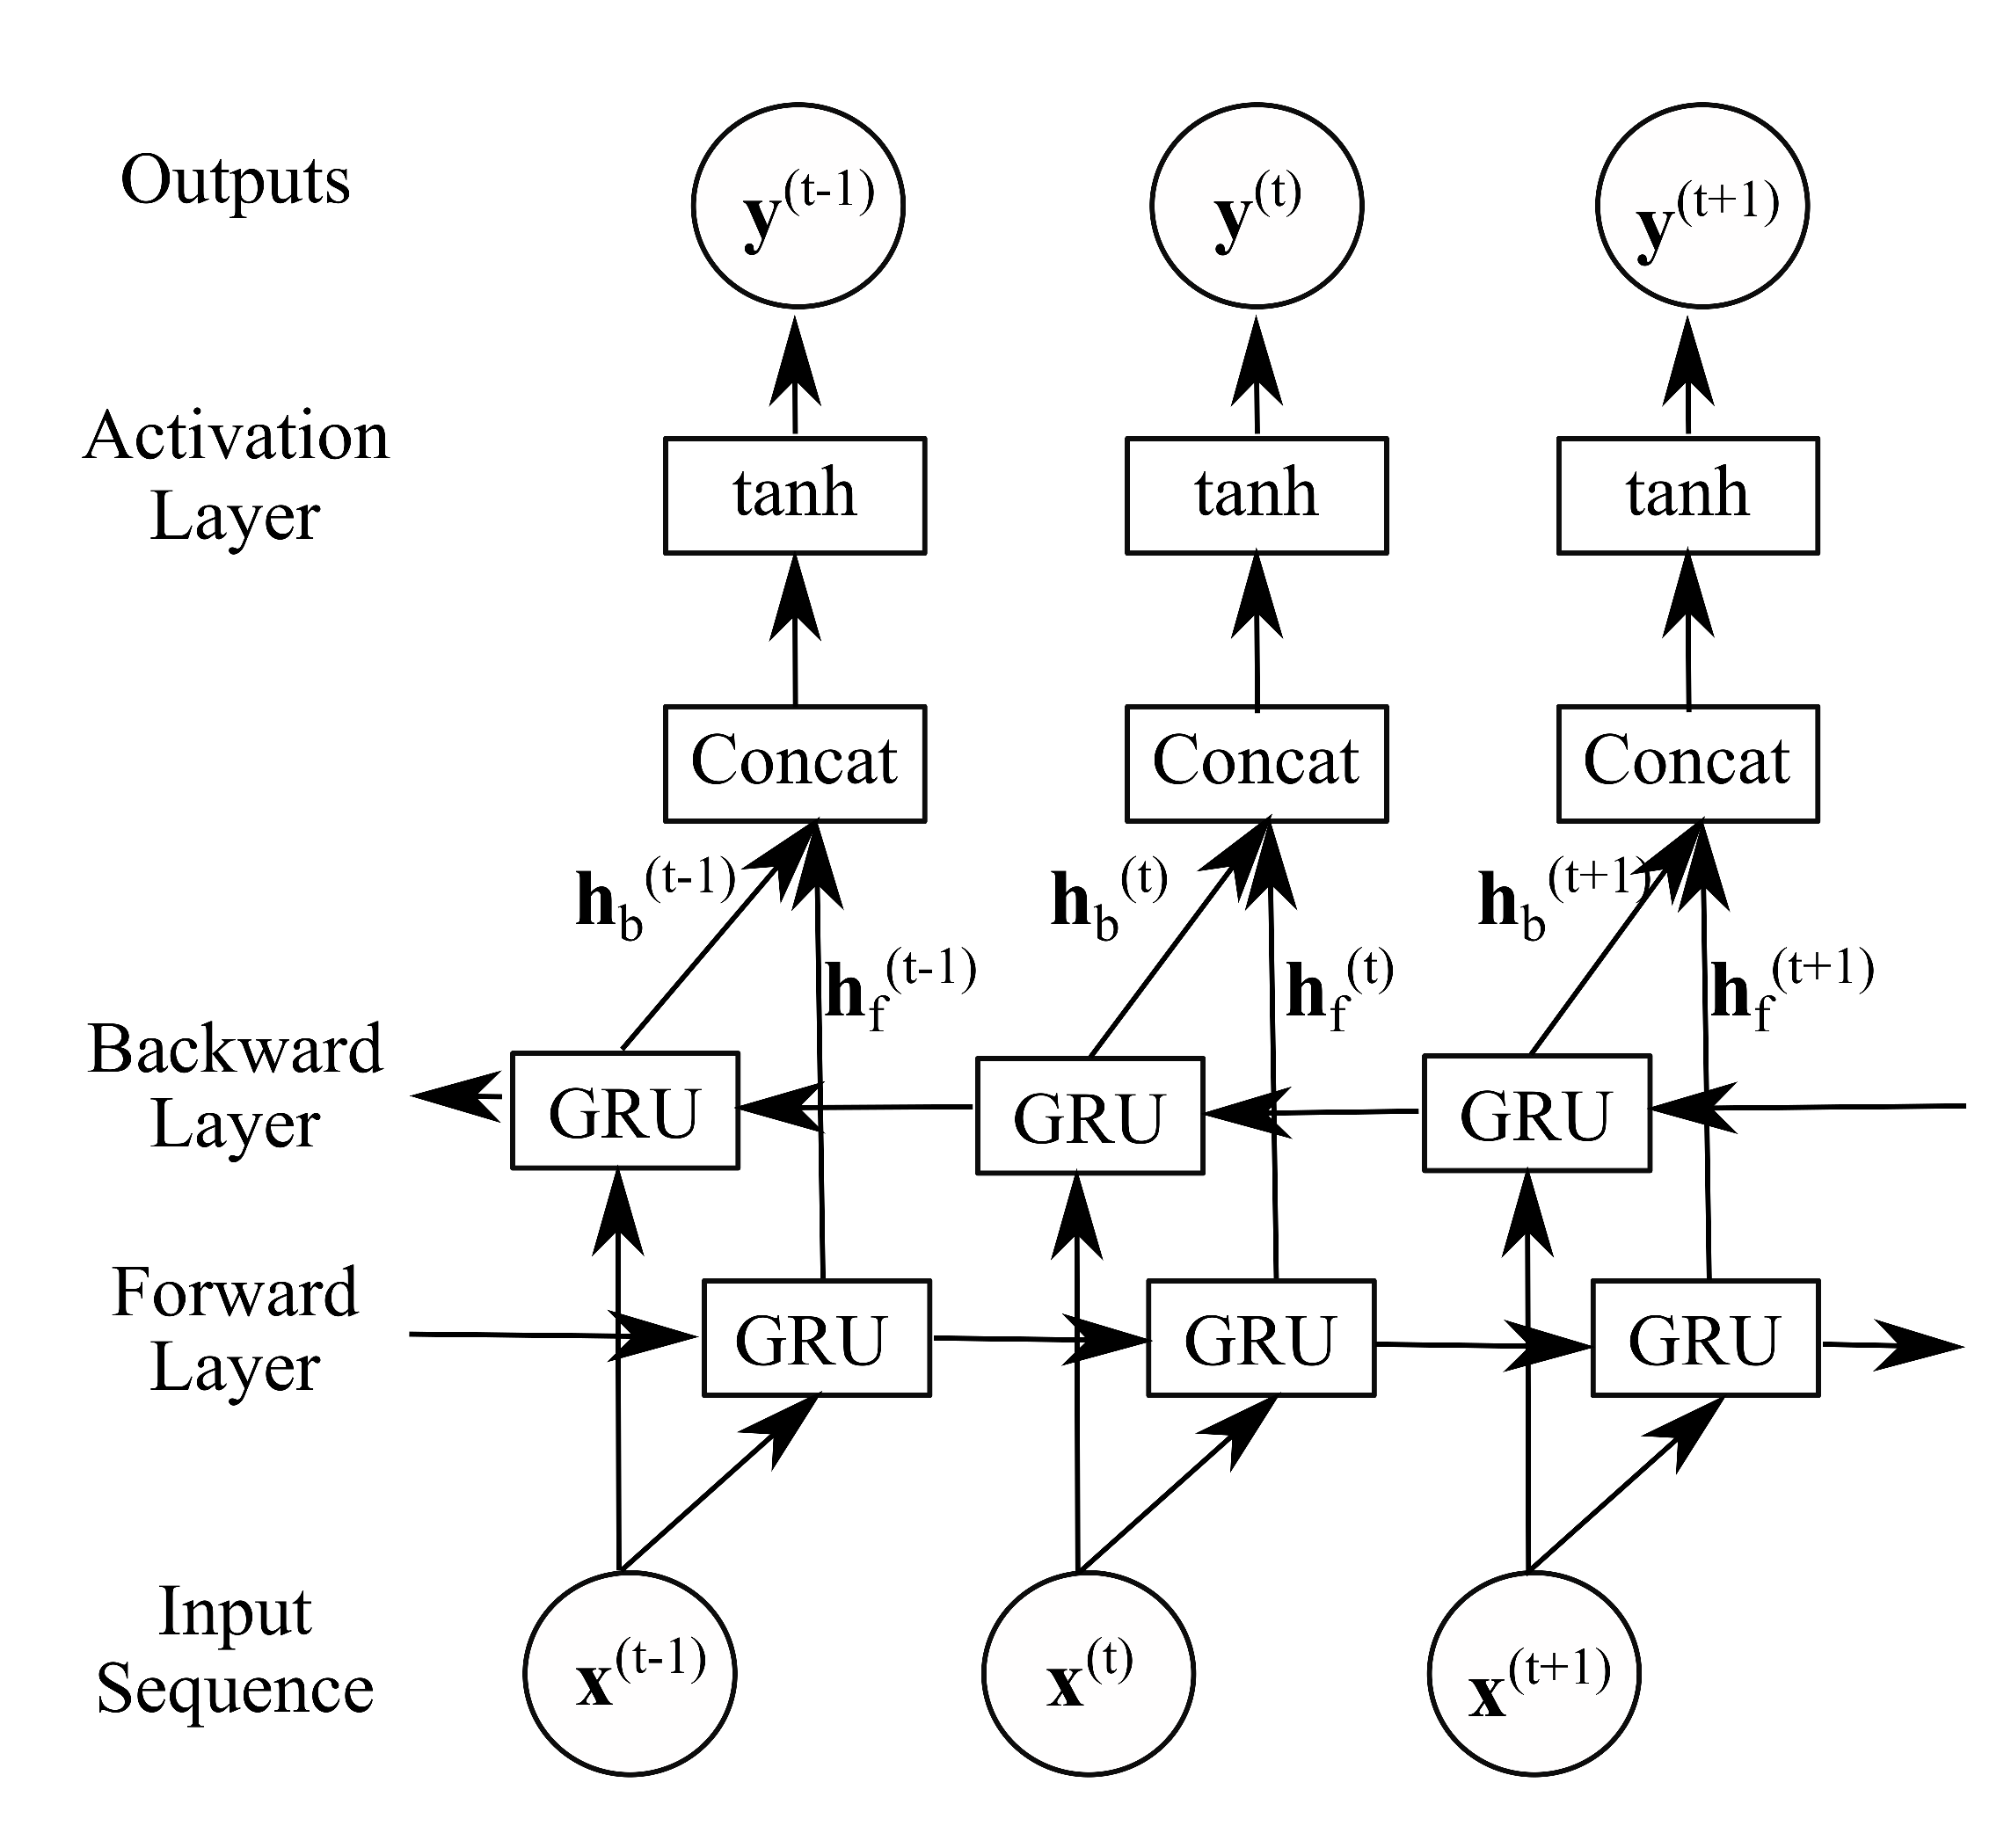
\includegraphics[width=0.7\textwidth]{figures/bigru.eps}
	\caption{The architecture of a bidirectional gated recurrent neural network \label{fig:bidirectional_gru}}
\end{figure}


\subsection{Regularization for Deep Learning}
Regularization is a technique which makes slight modifications to the learning algorithm such that the model generalizes better. This in turn improves the model's performance on the test data. As we know, \gls{dnn}s are highly complex models (many parameters and many non-linearities) and they are easy to overfit, hence, we need some form of regularization. Some of the very effective regularization techniques often employed in \gls{dnn}s training are discussed below.


\subsubsection{$L_{2}$ Regularization}
This type of regularization is popularly known as \textit{weight decay}. This strategy drives the weights closer to the origin. It works on assumption that smaller weights generate simpler model and thus helps to avoid overfitting. So, we can add an extra term to the loss expression in order to prefer solutions with smaller norms.

In $L_{2}$ regularization, regularization term is the sum of square of all feature weights. It forces the weights to be small but does not make them zero and does non sparse solution. This technique is also known as \textit{ridge regression}. It is expressed as: 

\begin{equation}
	\min_{w} {\sum_{t=1}^{N}l(\mathbf{f(x^{t}; W)}, y^{(t)}) + \lambda\sum_{i}\parallel{\mathbf{W}_{i}}\parallel_{F}^{2}}
\end{equation}
$\lambda$ is a parameter which controls the behavior of the regularization term. 


\subsubsection{Dropout}
Dropout is a computationally inexpensive but powerful regularization technique which prevents complex co-adaptations on training data in neural networks for reducing overfitting~\cite{Srivastava_14}. It is a very efficient way of performing model averaging with neural networks. The term \textit{dropout} refers to dropping out units (both hidden and visible) in a neural network. So, the key idea is to randomly drop units (along with their connections) from the neural network during training which prevents units from co-adapting too much. At test time, it is easy to approximate the effect of averaging the predictions of all these thinned networks by simply using a single unthinned network that has smaller weights. This significantly reduces overfitting and gives major improvements over other regularization methods. 


Another significant advantage of dropout is that it does not significantly limit the type of model or training procedure that can be used. It works well with nearly any model that uses a distributed representation and can be trained with stochastic gradient descent.


\subsubsection{Dataset Augmentation}
The simplest way to reduce overfitting is to increase the size of the training data. Therefore, we can collect more data or create fake data and add it to our training dataset. Explicit regularizer, such as weight decay and dropout, succeed in mitigating overfitting by blindly reducing the effective capacity of the model, implicit regularization such as dataset augmentation improves generalization by effectively capturing important characteristics of the data~\cite{Alex_18}. Furthermore, if the transformations are such that they reflect plausible variations of the real objects, it increases the robustness of the model. Besides, unlike explicit regularization techniques, data augmentation does not increase the computational complexity. It also transparently adapts to architectures of different depth, in contrast to  explicitly regularized models which need manual adjustment of the regularization parameters


\subsubsection{Early Stopping of Training}
One way to think of early stopping is as a very efficient hyperparameter selection algorithm. The idea of early stopping of training is that as soon as the validation error starts to increase we freeze the parameters and stop the training process. Or we can also store the copy of model parameters every time the error on the validation set improves and return these parameters when the training terminates rather than the latest parameters.

Early stopping has an advantage over weight decay that early stopping automatically determines the correct amount of regularization while weight decay requires many training experiments with different values of its hyperparameter.


\subsubsection{Noise Robustness}
Noise is often introduced to the inputs as a dataset augmentation strategy. The addition of noise with infinitesimal variance at the input of the model is equivalent to imposing a  penalty on the norm of the weights. Noise injection is much more powerful than simply shrinking the parameters. 

In addition to adding noise to the inputs, random noise can be added to the other parts of the network during training. 
The addition of the noise to the layer activations can be useful for deep networks as it allows noise to be used at any point in the network. Again, noise can be added to the layer outputs themselves, but it more likely achieved via the use of noisy activation function. Another way that noise has been used in the service of regularizing models is by adding it to the weights. This technique has been employed primarily in the context of recurrent neural networks. This can be interpreted as a stochastic implementation of Bayesian inference over the weights~\cite{Goodfellow_16}.



\subsection{Normalization}
Normalizing the input data of neural networks to zero-mean and constant standard deviation has been known for decades to be beneficial for neural network training. Batch normalization (\gls{bn})~\cite{Ioffe_15} is a technique to normalize activations in intermediate layers  of \gls{dnn}s across the mini-batch.   Its tendency to improve accuracy and speed up training have established \gls{bn} as a favorite technique in deep learning. For each feature, batch normalization computes the mean and variance of that feature in the mini-batch. It then subtracts the mean and divides the feature by its mini-batch standard deviation. This restricts the activations to have $0$ mean and unit standard deviation.

Given $N$ input samples each denoted by a vector $x^{(i)}\epsilon~~\mathbb {R}^d,~~~i = 1, . . . , N$, BN computes the mean and variance of each dimension independently across all the samples.

\begin{equation}
	\begin{split}
	  \mu_{j} &= \frac{1}{N}\sum_{i=1}^{N}x{j}^{i}~~~~~~~~~~~~~~~~~~~[minibatch~mean] \\
	  \sigma_{B}^{2} &= \frac{1}{m}\sum_{i=1}^{m}{(x_{i}-\mu_{B})}^2~~~~~~[minibatch~variance]
	\end{split}
\end{equation}

Then it normalizes the input to be zero mean and unit variance by
\begin{equation}
\hat{x}_{j}^{(i)} = \frac{x_{j}^{(i)} - \mu_{j}}{\sqrt{\sigma_{j}^2+\epsilon}} ~~~~~~~~~[normalize]
\end{equation}

where $\epsilon$ is a small positive number that avoids zero division. At last, BN applies a linear transformation to $\hat{x}$ by
\begin{equation}
~~~~~~~~~~~~~y_{j}^{(i)}  = \alpha_{j}\hat{x}_{j}^{(i)} + \beta_{j}~~~~[scale~and~shift]
\end{equation}
where $\alpha,~\beta~\epsilon~~\mathbb {R}^d$ are learnable parameters.



%.....................................................................................................
\section{Human Pose Estimation} \label{sec:pose_estimation}
Human pose estimation, one of the core problems in computer vision, refers to the process of inferring poses in an image or video. Essentially, it entails predicting the body parts or body joint positions of individuals in an image.
It is the key component which enables machines to have a perception of the people in images and videos. It has been successfully employed in many real-world applications such as action recognition~\cite{Song_17}, augmented reality~\cite{Marchand_16}, gaming~\cite{Ke_10}, and gait recognition~\cite{Liao_19}. 


\subsection{Types of Pose Estimation} 
Depending upon the output dimension requirement, a pose estimation algorithm can be categorized into 2D pose estimation and 3D pose estimation. In 2D pose estimation, the location of the body joint is predicted in terms of pixel values of the image frame. On the other hand, 3D pose estimation is predicting a three-dimensional spatial arrangement of all the body joints as its final output. Again, depending on the number of people being tracked, pose estimation can be further classified into single-person and multi-person. Single-person pose estimation guarantees of only one person present in the frame, whereas, in multi-person pose estimation, each image may contain an unknown number of people who can appear at any position or scale. Therefore, it needs to handle the additional problem of inter-person occlusion. 

\begin{figure}[t]
	\centering
	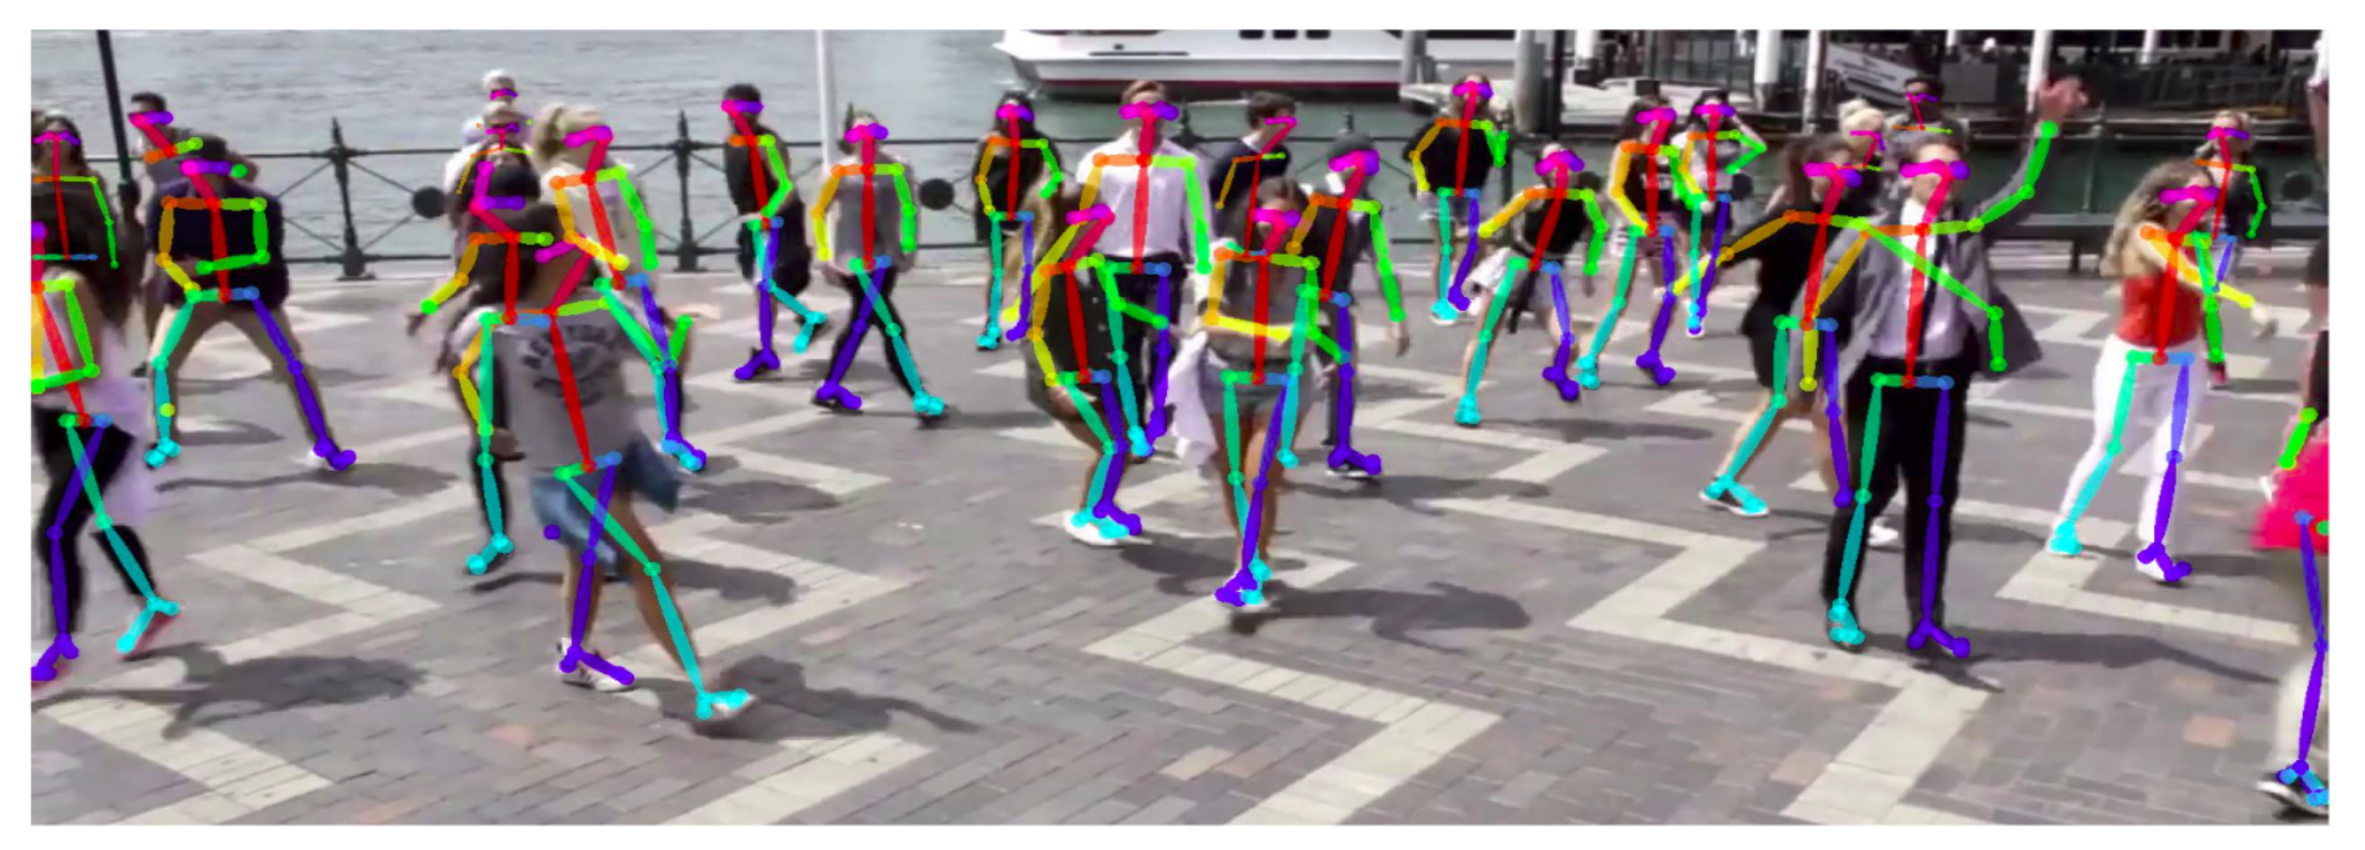
\includegraphics[width=\textwidth]{figures/openpose_demo.eps}
	\caption[Realtime multi-person 2D pose estimation using OpenPose algorithm]
	{Realtime multi-person 2D pose estimation using OpenPose algorithm. [Image courtesy Cao et al.~\cite{Cao_19}] \label{fig:openpose_demo}}
\end{figure}


\subsection{Techniques for Pose Estimation} 
There are two overarching approaches to pose estimation: a \textit{bottom-up} approach, and a \textit{top-down }approach.

With a bottom-up approach, the model detects every instance of a particular keypoint in a given image and then attempts to assemble groups of keypoints into skeletons for distinct objects. In simpler terms, the algorithm first predicts all body joints present in the image. This is typically followed by the formulation of a graph, based on the body model, which connects joints belonging to the same human. Integer linear programming (ILP) or bipartite matching are two common methods of creating this graph.

While, a top-down approach involves a segmentation step at the start. The network first uses an object detector to draw a box around each instance of an object and then estimates the keypoints within each cropped region. 

The potential simplest model for pose estimation used \gls{dnn}-based regressor to predict X, Y, and potentially Z coordinates for each keypoint location from an input image. In practice, however, this architecture does not produce accurate results without additional refinement. 

A slightly more complicated approach employs a deep learning-based encoder-decoder architecture. In this type of approach, instead of estimating the keypoint coordinates directly, the encoder is fed into a decoder, which creates heatmaps representing the likelihood that a keypoint is found in a given region of an image. During post-processing, the exact coordinates of a keypoint are found by selecting heatmap locations with the highest keypoint likelihood. In the case of multi-pose estimation, a heatmap may contain multiple areas of high keypoint likelihood (e.g. multiple right hands in an image). 

In top-down approach, an object detection module is placed between the encoder and decoder which is used to crop regions of an image likely to contain an object. Keypoint heatmaps are then predicted individually for each box. Rather than having a single heatmap containing the likely location of all of the specific body part in an image, we get a series of bounding boxes that should only contain a single keypoint of each type. 

So, top-down approach makes it easy to assign the keypoints to specific instances without a lot of post-processing. However, it suffers greatly when the person detector fails due to close proximity among people. Furthermore, their runtime is proportional to the number of people in the image. Contrarily, bottom-up approaches show robustness to early commitment and have the potential to decouple runtime complexity from the number of people in the image~\cite{Cao_19}.



\subsection{Introduction to OpenPose Library} 
\begin{figure}
	\centering
	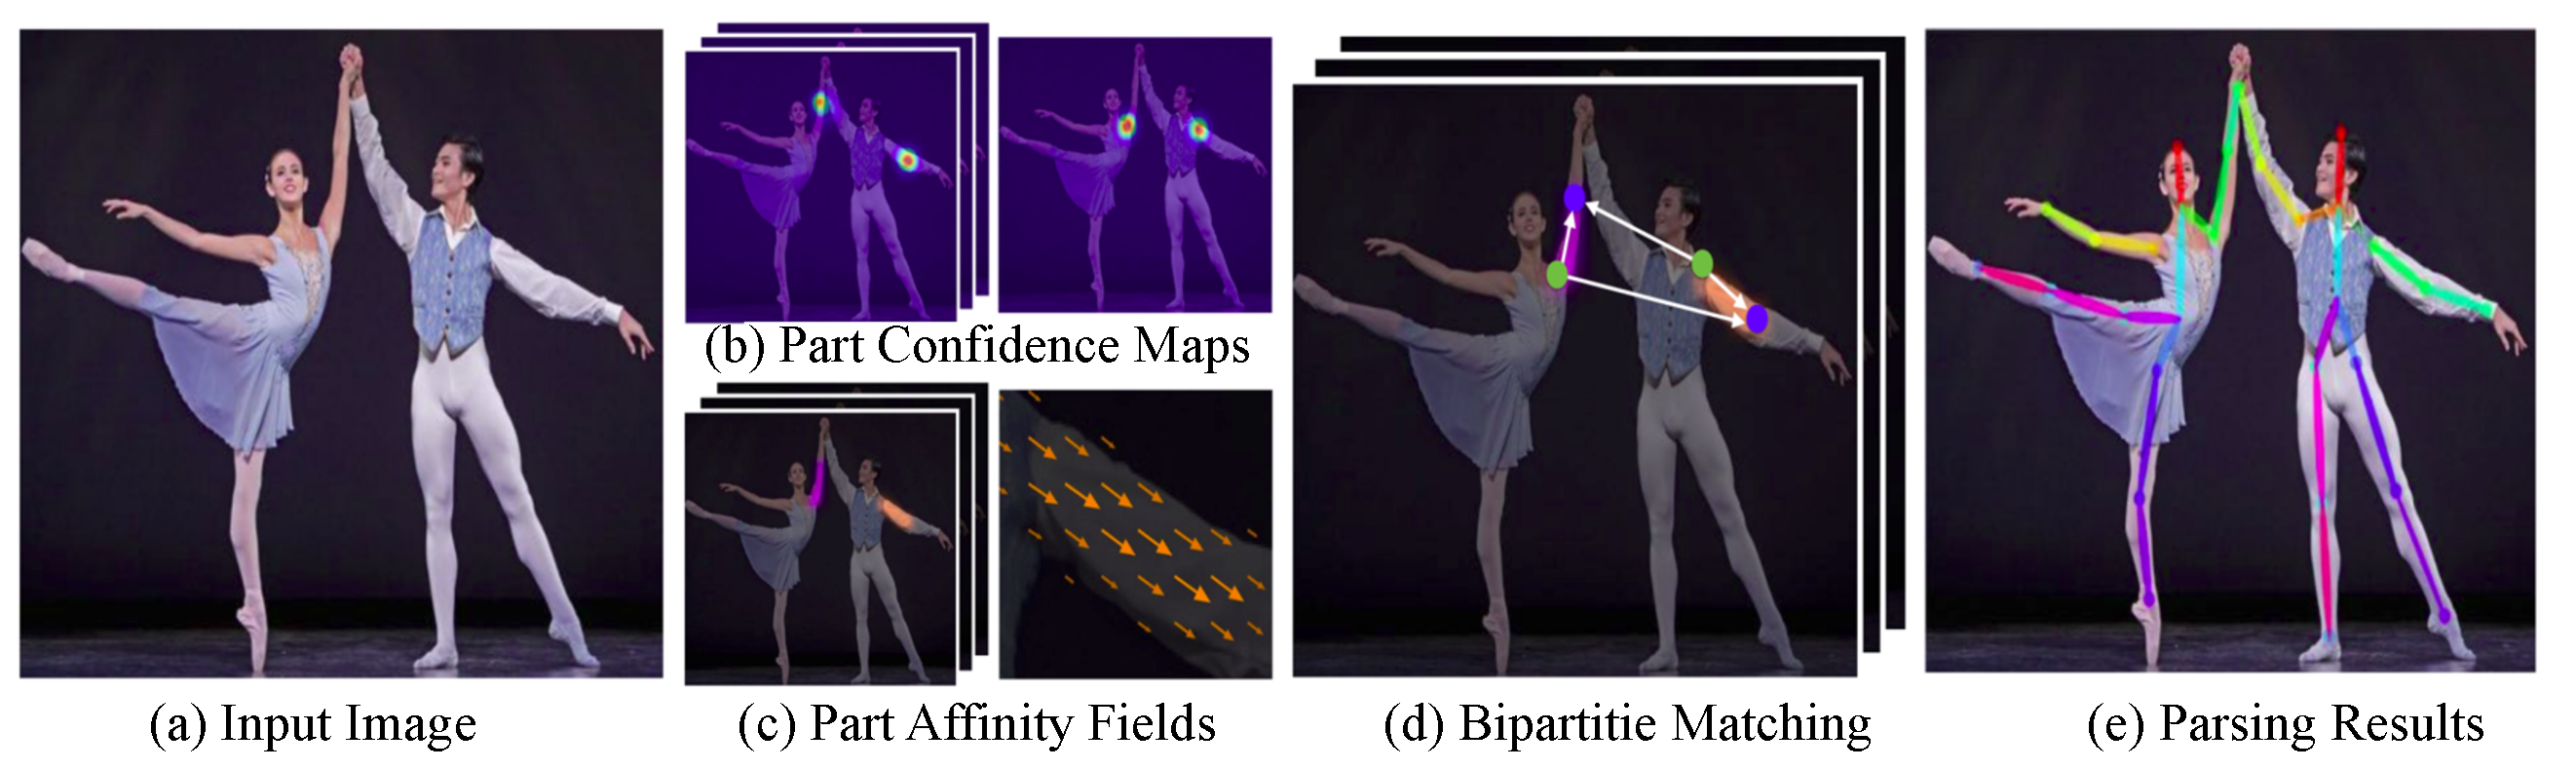
\includegraphics[width=\textwidth]{figures/openpose_bottom_up.eps}
	\caption[An example of a bottom up approach]
	{An example of a bottom up approach. [Image courtesy Cao et al.~\cite{Cao_19}] \label{fig:openpose_bottom_up}}
\end{figure}

\begin{figure}
	\centering
	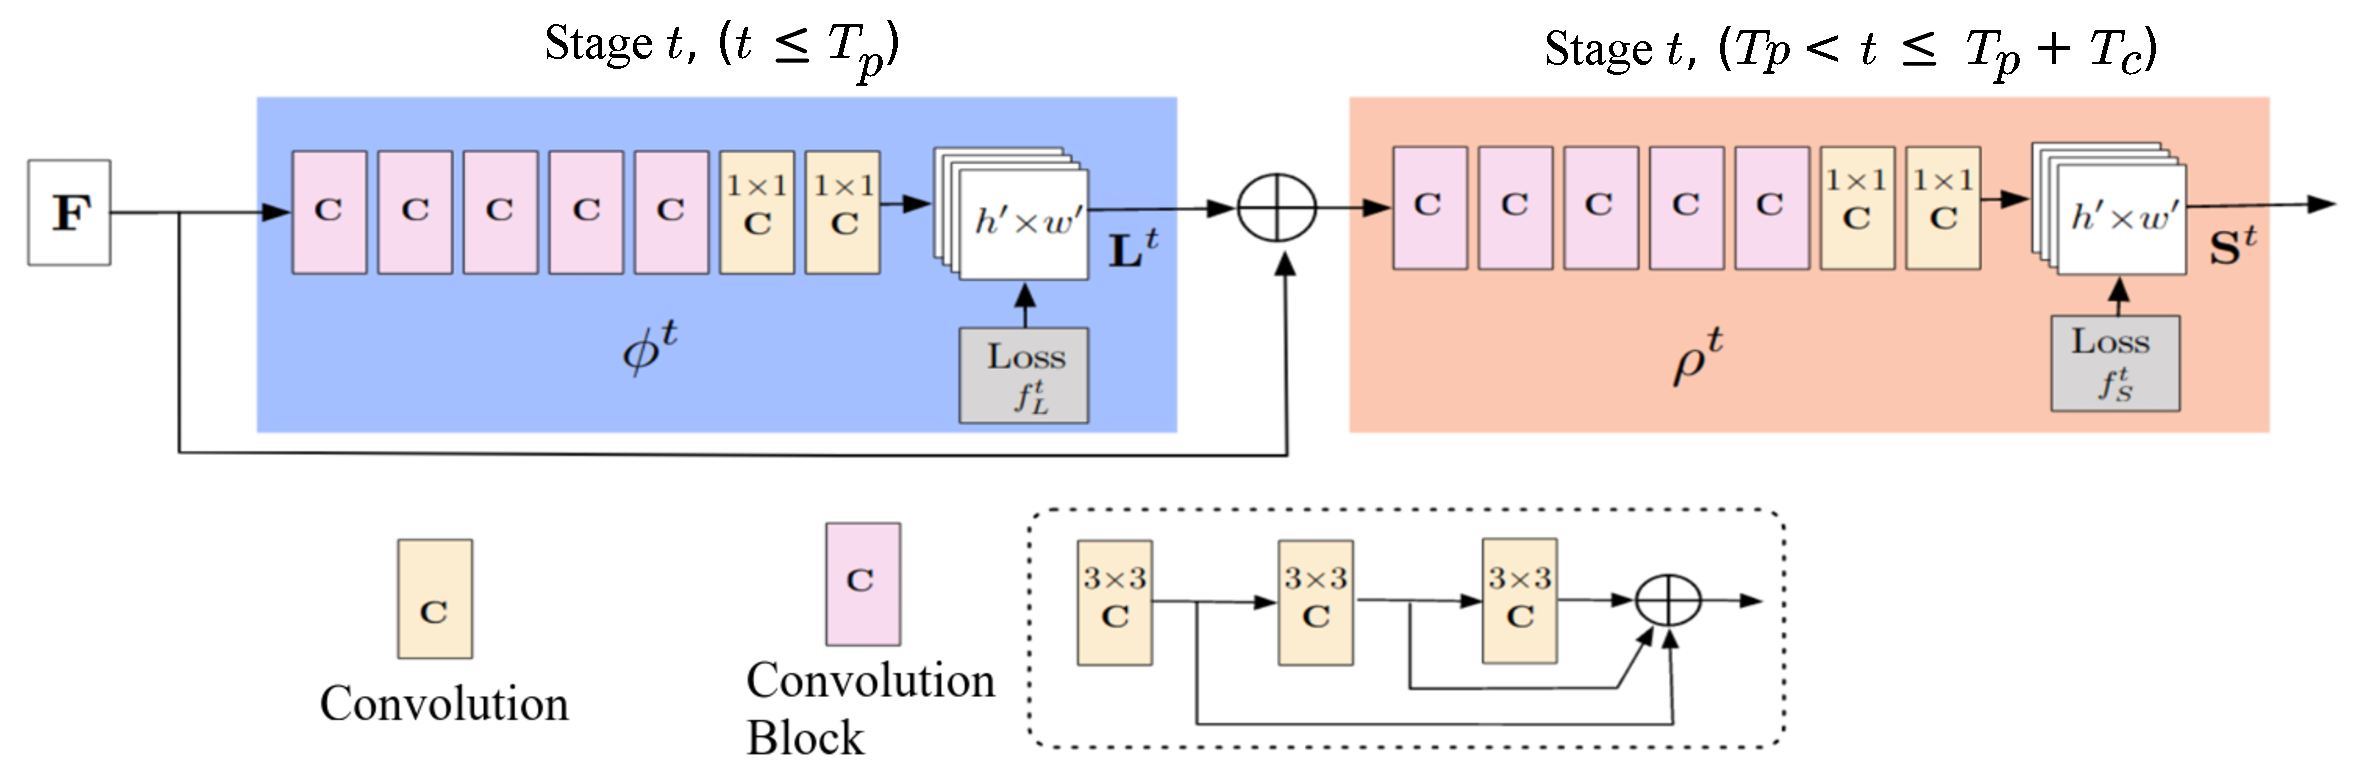
\includegraphics[width=\textwidth]{figures/openpose_architecture.eps}
	\caption[Network architecture of the multi-stage CNN]
	{Network architecture  of  the  multi-stage  CNN.  The  first  set of stages predicts PAFs $\textbf{L}^t$, while the last set predicts confidence  maps $ \textbf{S}^{t}$. [Image courtesy Cao et al.~\cite{Cao_19}] \label{fig:openpose_architecture}}
\end{figure}

In this research, we have employed OpenPose~\cite{Cao_19}, an open-source library for realtime multi-person 2D pose detection including body, foot, hand, and facial keypoints. This bottom-up approach achieves state-of-the-art accuracy in realtime performance. 

The overall pipeline of the OpenPose library is illustrated in Figure~\ref{fig:openpose_bottom_up}. An RGB image(Figure~\ref{fig:openpose_bottom_up}a) is fed as input to the library and it outputs the 2D locations of anatomical keypoints for each person in the image (Figure~\ref{fig:openpose_bottom_up}e). Firstly, a feedforward network predicts a set of 2D confidence maps \textbf{S} of body part locations (Figure ~\ref{fig:openpose_bottom_up}b) and a set of 2D vector fields \textbf{L} of part affinity fields (PAFs), which encode the degree of association between parts (Fig. ~\ref{fig:openpose_bottom_up}c). The set $\textbf{S} = (\textbf{S}_1,\textbf{S}_2,...,\textbf{S}_J)$ has $ J $ confidence maps, one per part, where $\textbf{S}_j~\epsilon \mathbb~{R}^{w\times h}$ . The set $\textbf{L}= (\textbf{L}_1,\textbf{L}_2,...,\textbf{L}_C)$ has C vector fields, one per limb, where $\textbf{L}_c~\epsilon~\mathbb {R}^{w\times h\times 2}$. Each image location in $\textbf{L}_c$ encodes a 2D vector. Finally, the confidence maps and the PAFs are parsed by greedy inference (Figure ~\ref{fig:openpose_bottom_up}d) to output the 2D keypoints for all people in the image. The network architecture of OpenPose algorithm, shown in Figure~\ref{fig:openpose_architecture}, iteratively predicts affinity fields that  encode part-to-part association.
